\section{FindingPlaces}\label{sec:findingplaces}
{
    \subsection{Introduction}

    {
        In late 2015, a few months after the completion of the BRT project \eqref{sec:brt}, CityScope was again proposed as a way to construct consensus, in this case for the intensifying refugees crisis in northern Europe. \textit{``FindingPlaces''} (FP) was a city-wide public engagement process that was created for the allocation of housing accommodation for thousands of refugee in the City of Hamburg, Germany. CityScope was in the center of the FindingPlaces process, offering a socio-technical solution to facilitate effective interaction between participants and stakeholder groups. Between May and July 2016, 34 workshops were held with nearly 400 participants, resulting with 161 sites being allocated for refugee housing all around Hamburg's metro area. Following its completion, FP was awarded the UN-URBACT Good Practice Award (2017) \cite{urbact:online}, named Global Innovation by the OECD Observatory for Public Sector Innovation (OPSI) and the Centre for Government Innovation (MBRCGI) (2018) \cite{opsi:online}, and was exhibited at the Edge of Government summit in Dubai (2019) \cite{EdgeofGo35:online}. Site founded during FP are still in use by the City of Hamburg for current, as well as future refugee housing needs.
    }

    \begin{figure}[!htb]
        \begin{center}
            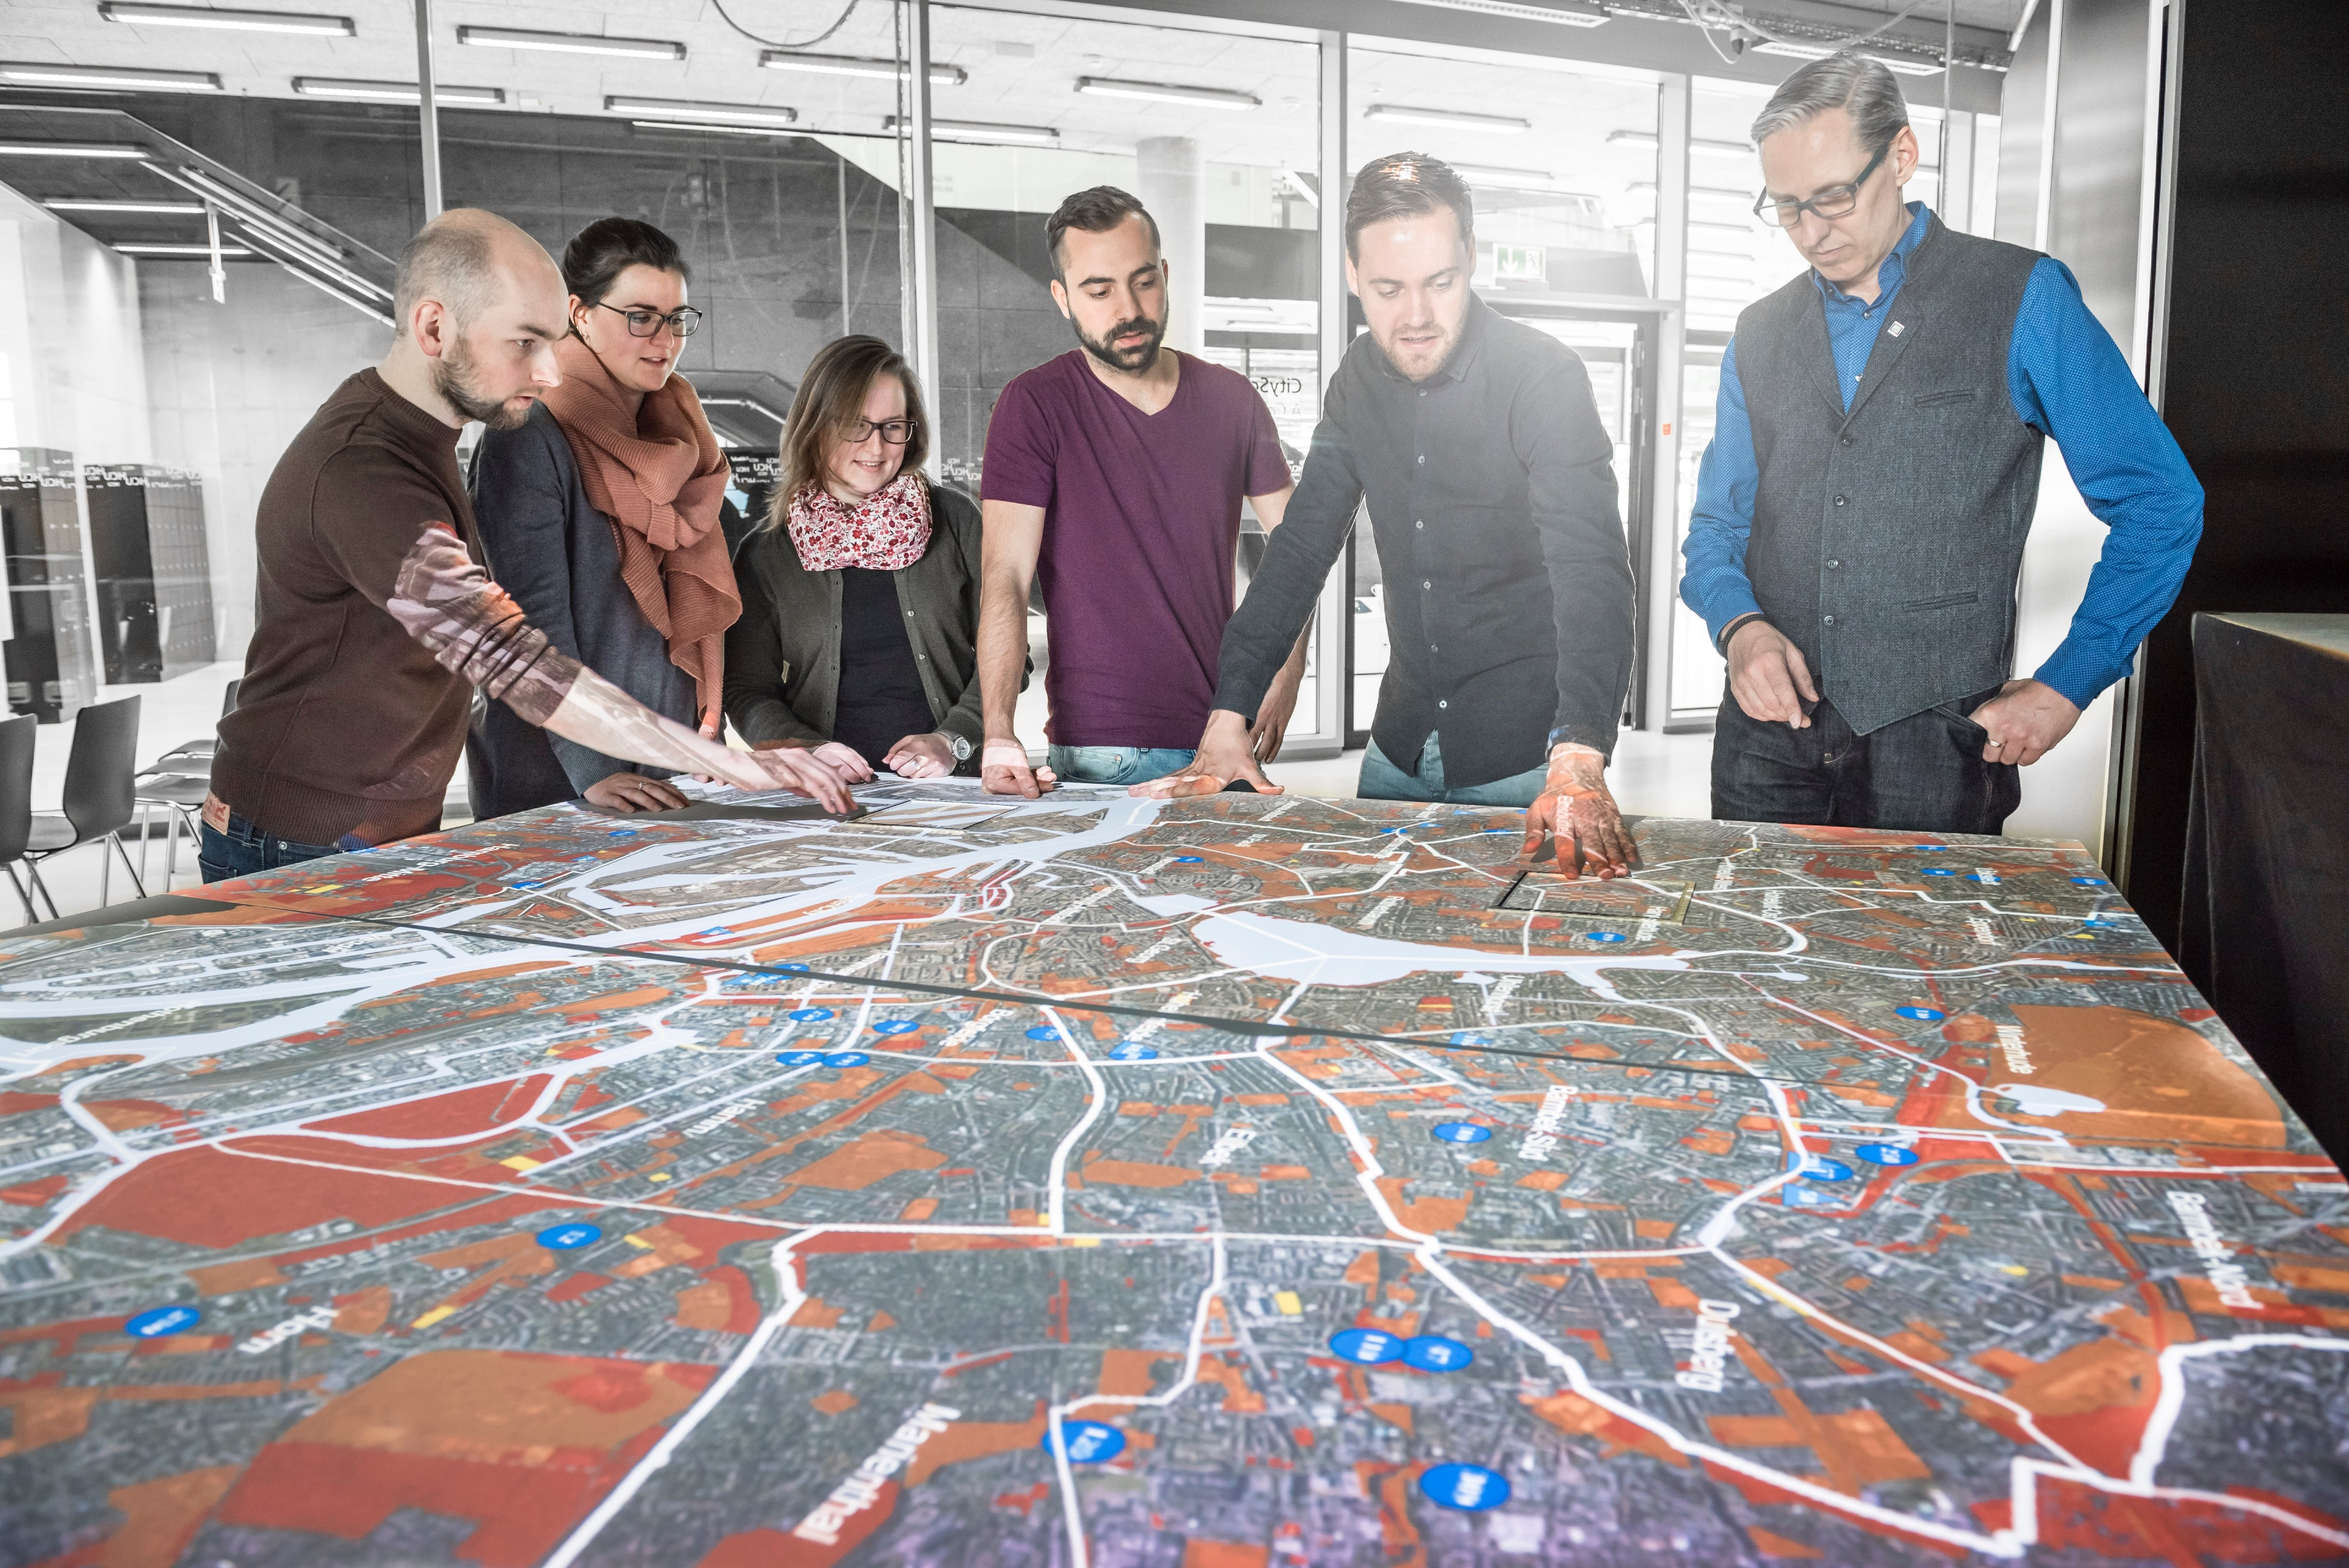
\includegraphics[width=1\textwidth]{chapters/consensus/findingplaces/figures/fp0.jpg}
        \end{center}
        \caption{A Typical FindingPlaces session. Groups of up to 20 participants were gathered in the HCU campus; After an introduction, participants were asked to use the first CityScope table, in order to discuss the current state of refugee accommodation in Hamburg (noticeable as blue dots). Additionally, they were introduced to the spatial limitations of accommodations in certain vacant areas, such as parks, playgrounds, and sports fields (marked in different hues of red). Photo: W. Schieswohl, HCU}
        \label{fig:fp_session}
    \end{figure}

    \subsection{Europe's Refugees Crisis}

    {
        Approximately 21 million refugees fled their home countries in 2015. A total number of 1.2 million applications for asylum were filed in Europe, more than 300\% than the previous year. As the European Union struggled to determine to accommodate refugees, disparities emerged within the member states: Germany received more than a third of the asylum applications (442,000), more than any other member state \cite{fur2015fluchtlinge}. The persistent influx of asylum seekers posed major risks to German federal states and municipalities. As a consequence, ad-hoc solution were hastily implemented, and in many cases, refugees were accommodated in tents, warehouses or gymnasiums \cite{katz2016cities}. The limitation in space for refugee accommodation represented a major obstacle for a long-term planning process, especially in densely built cities and rapidly growing urban regions. Many cities have failed to guarantee fair and equal distribution of refugees within their bounds, and instead opted to utilize temporary solutions, such as refugee camps \cite{MISSINGM99:online}. Figure \ref{fig:fp_refugees_housing} shows the situation of refugee accommodation in Germany, 2015.

        \begin{figure}[!htb]
            \begin{center}
                \includegraphics[width=1\textwidth]{chapters/consensus/findingplaces/figures/fp4.png}
            \end{center}
            \caption{
                Refugees in Germany, 2015. The influx of refugees and asylum-seekers during `15-`16 brought the German Government and local municipalities to seek quick solutions: Under-used facilitates, such as Berlin's Tempelhof Airport, were transformed into refugee camps; In Hamburg, tent-cities were constructed and empty properties were re-used in an effort to accommodate thousands of refugees. In most cases, these solutions could only offer short-term remedy, but were not suitable as long-term accommodations. Photo: C. Charisus, DW.com
            }
            \label{fig:fp_refugees_housing}
        \end{figure}


        In Hamburg, accommodation facilities concentrated in certain neighborhoods, while others received little to no refugees at all. Civil protest against refugee accommodation projects began to arise. Only few cases of physical hostility towards foreigners were reported, but nevertheless highlighted the civics' demand to be heard \cite{Antiraci26:online}. The heated and emotional debate motivated Hamburg's First Mayor to initiate a citizen dialogue and openly discuss where-and-how to accommodate refugees now and in the future. The idea was to address the issue as a collective, in which citizens themselves could take responsibility and contribute their knowledge towards a common solution. This participation process was given the name ``FindingPlaces'' (FP) \cite{Hamburge78:online}.
    }

    \subsection{Political Mandate and Goals}
    {

        \begin{figure}[!htb]
            \begin{center}
                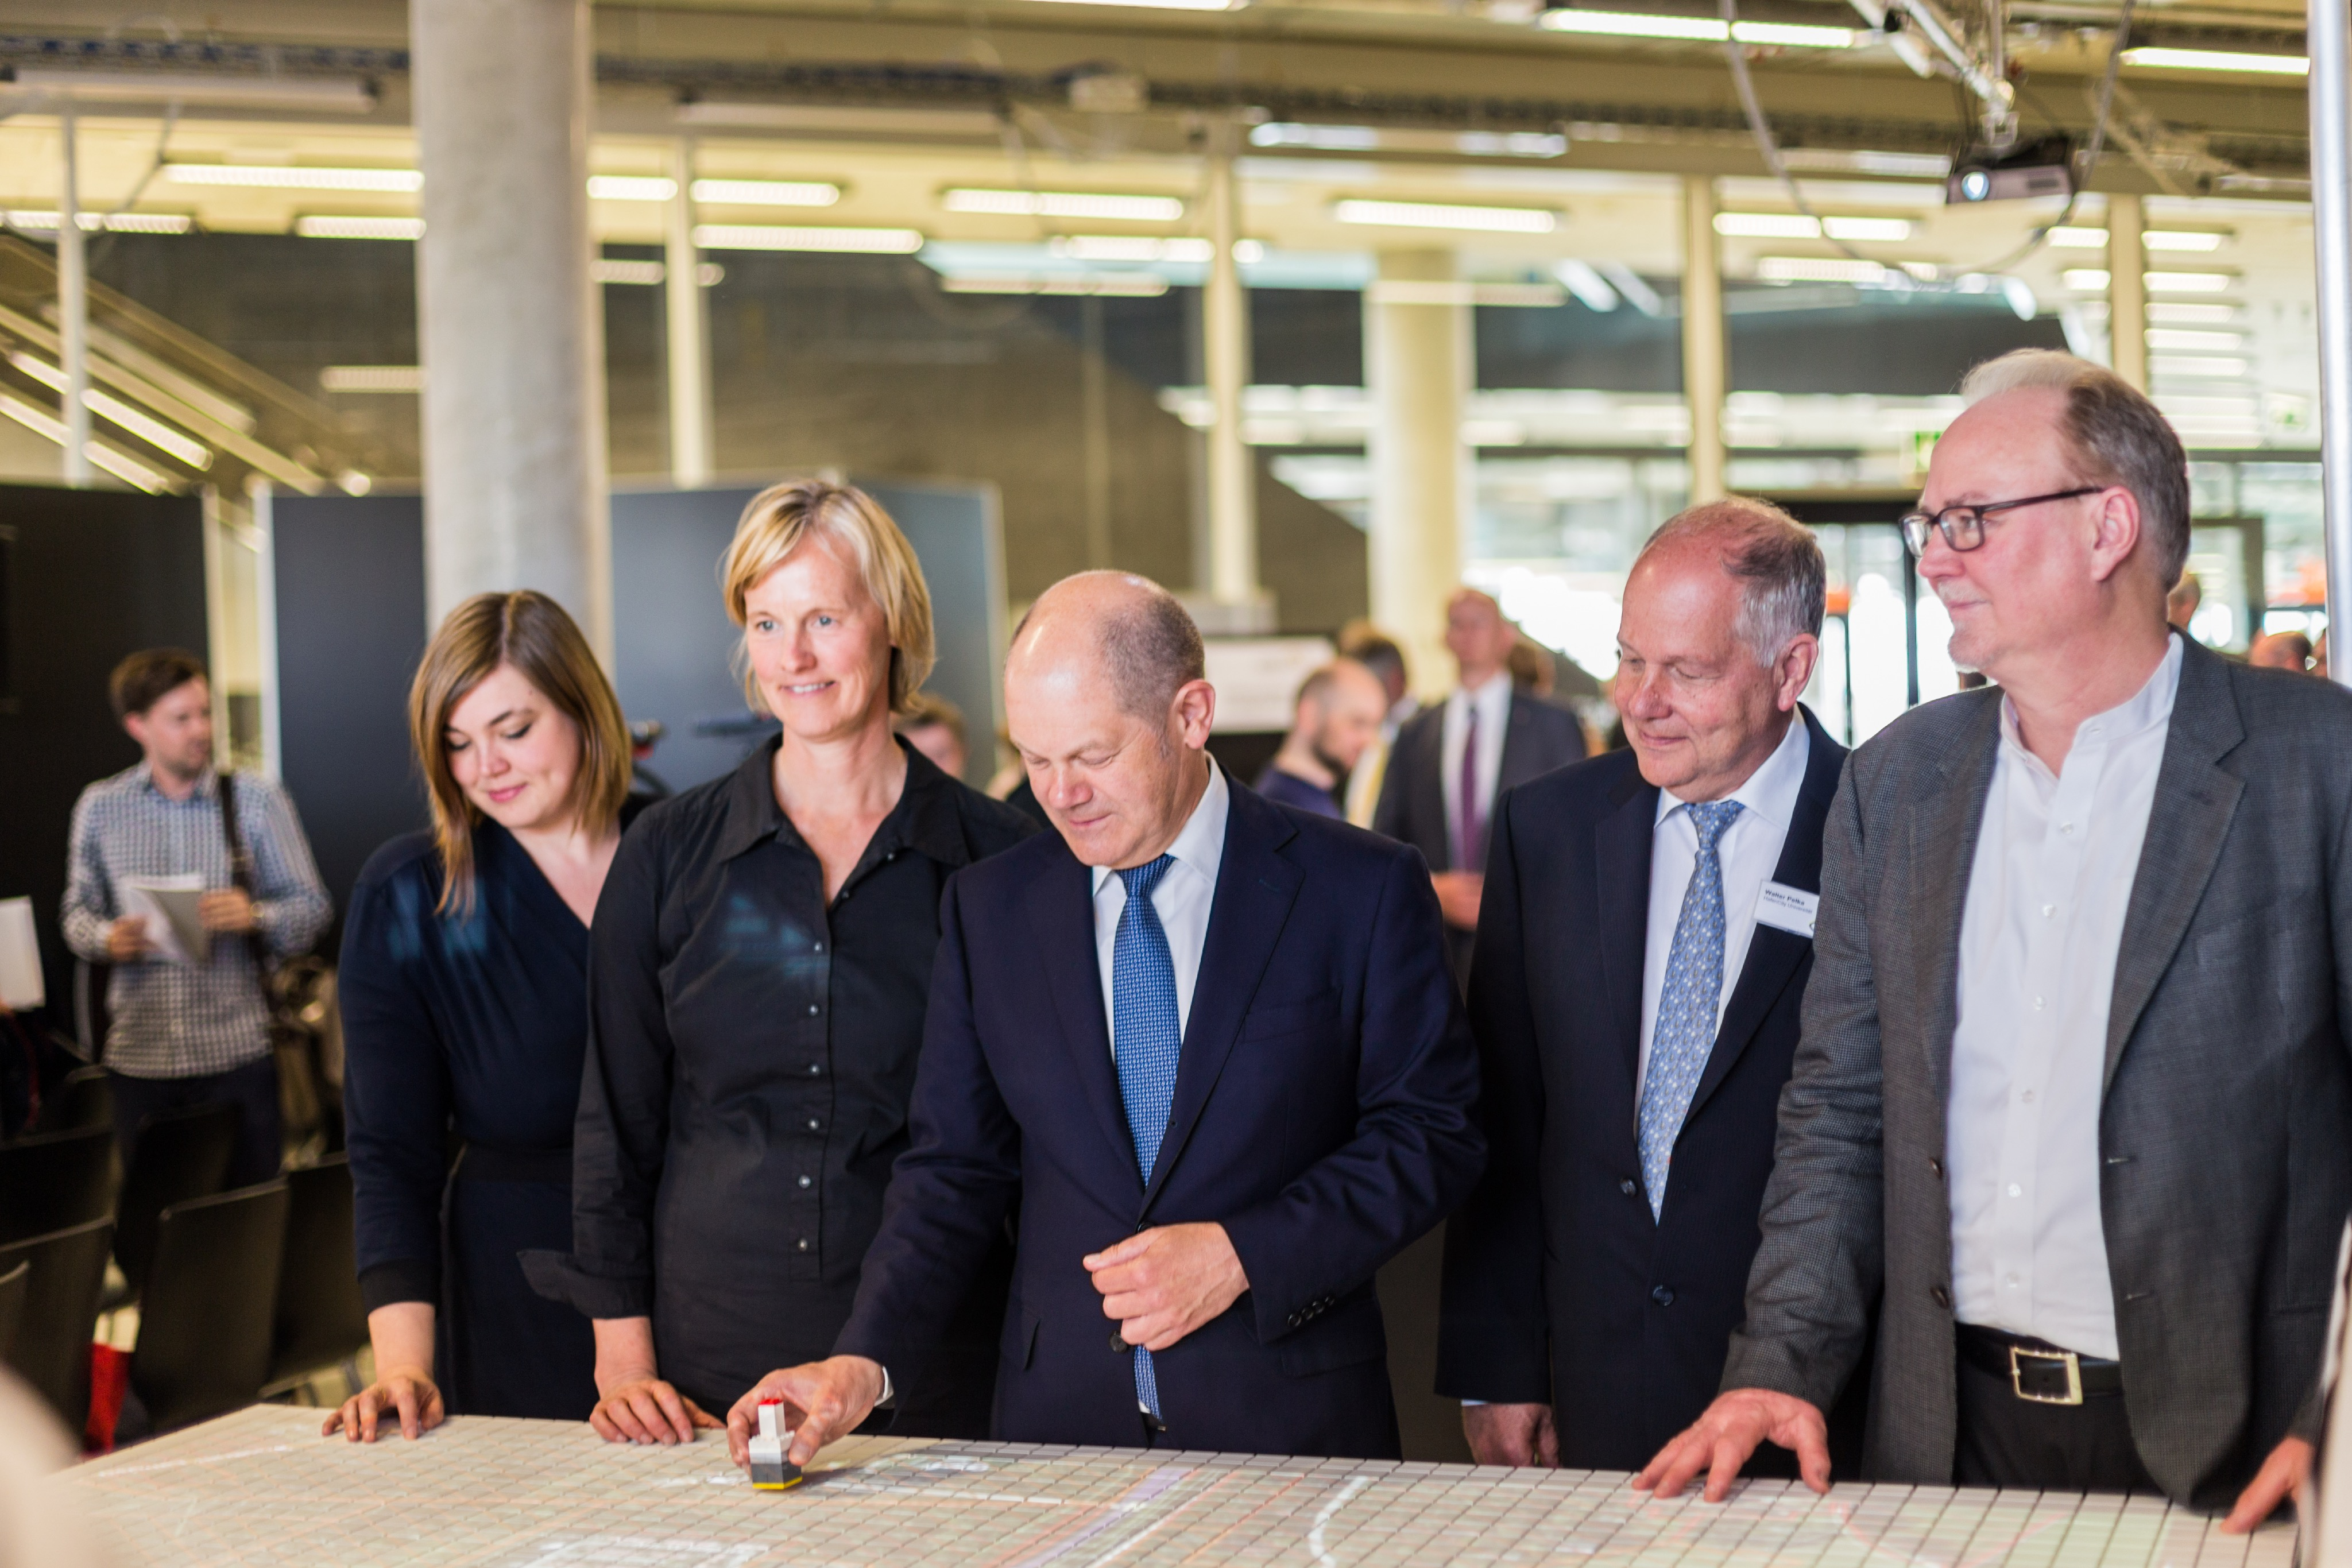
\includegraphics[width=1\textwidth]{chapters/consensus/findingplaces/figures/fp6.jpg}
            \end{center}
            \caption{
                Inaugurating FindingPlaces. On May 11\textsuperscript{th} 2016, Olaf Scholz, (First Mayor of Hamburg `11-`18, Chancellor of Germany since `21), inaugurated the project and invited the public to take active role in setting their city's future: \textit{``FindingPlaces brings together the knowledge of residents, authorities and geographers and makes it immediately usable. The participants in the workshops are in the position of informed city planners who have to deal with an extremely complex task. It's not just any theoretical task, but the task that our city has to solve together: Which areas can we use to house refugees? FindingPlaces answers: This is your city! Here is your chance to examine whether what makes sense in theory, is also suitable in practice.''} (Excerpts from Olaf Scholz's speech, May 11\textsuperscript{th} `16, HCU) Also in this photo (from left to right): Katharina Fegebank, Second Mayor of Hamburg; Prof. Dr. Gesa Ziemer HafenCity Universität, Director CSL; Olaf Scholz, 1\textsuperscript{th} Mayor of Hamburg; Walter Pelka, frmr. HCU President; and Kent Larson, Dir. MIT City Science.
            }
            \label{fig:fp_olaf_scholz}
        \end{figure}


        In June 2015, The City of Hamburg and the MIT Media Lab signed a long-term research collaboration agreement that promoted the establishment of the City Science Lab (CSL) at HafenCity University Hamburg (HCU) \cite{HafenCit25:online}. In February 2016, CSL was assigned by then First Mayor Mayor Scholz\footnote{As of Dec. `21, Olaf Scholz is new German Chancellor, succeeding Angela Merkel} to develop a participatory process that would enable citizens to engage in finding accommodations for a predicted influx of nearly 80,000 refugees. The goal was to incorporate the citizens' personal experience and local knowledge into the political and administrative evaluation of potential locations, while creating a public discourse, innovation, and learning around the challenges of immigration. The results and proposals emerging from the participation process were to become recommendations for decision-makers and planning authorities. FP was developed in coordination with the Senate Office, the Central Refugees Coordination Staff (ZKF)\footnote{\url{https://www.hamburg.de/sfa-about-us/}}, district administration representatives, and the Hamburg Urban Development and Revitalization Agency (STEG)\footnote{\url{https://www.steg-hamburg.de/}}, who specialized in citizen participation processes. The mayor's office permitted three months for conception and development of FP. Figure \ref{fig:fp_olaf_scholz} shows the inauguration event of FindingPlaces by the First Mayor of Hamburg.
    }

    \subsection{Concept and Method}
    {
        Traditionally, decision-making for the allocation of refugees accommodations was mostly done by small groups of experts based on their technical, legal, and contextual knowledge \cite{sprandel2018housing}. FP required multidisciplinary expertise and methods to tackle the question of citizens' involvement in refugees' accommodations. To enable citizens' input, CityScope was proposed as a decision-making and knowledge-support tool, that can leverage the publics' insights in concert with evidence-based urban data, analytics, and predictions. A series of public participation workshops was planned to be centered around interactive CityScope stations, displaying data to citizen groups as they worked out decisions. The main conceptual components of FP included (i) A workflow design for the overall workshop series; (ii) A procedure for participatory workshops; (iii) The technical adaptation of CityScope interactive tools; and (iv) Extensive pre-processing of urban data.
    }

    \subsection{System Design}
    {
        The FP use-case presented a set of unfamiliar socio-technical challenges. Adaption of the CityScope to FP required major refactoring of the system, such as the introduction of networked communication between platforms, integration of a real-time Geographic Information System (GIS) service, as well as streamlined data , stability, and error mitigation. Workshops were designed to focus on one interactive CityScope table at a time, showing a user-selected part of the city on a scale of $1:750m$. Geographic data on Hamburg's parcels were augmented by several data layers, such as ownership models, land-use, environmental conditions, or hazards, to highlight places' suitability for refugee accommodation.

        \subsubsection{Data}
        {
            To evaluate the availability of a parcel for refugee accommodation, detailed information about Hamburg's land uses and land distribution was required. Different spatial data sources were aggregated into the GIS database, such as parcels ownership model, current uses of parcels, and existing development constraints, such as nature reserves or land contamination. These geospatial layers were sorted into three ranked classes:

            \begin{itemize}
                \item{
                            \textbf{High indication of unsuitability}: Places significantly affected by highly restrictive criteria, such as nature conservation, cemeteries, places under significant noise emission, etc.
                      }
                \item{
                            \textbf{Medium indication of unsuitability}: Places insignificantly affected of aforementioned highly restrictive criteria but still affected by less restrictive criteria like parks, designated recreational areas, proximity to high-voltage power lines or similar.
                      }
                \item{
                            \textbf{Low or no indication of unsuitability}: Places not affected by highly restrictive criteria with less restrictive criteria affecting less than 50\% of the area.
                      }

            \end{itemize}
            These classes were set to provide a baseline for the selection of places discussed during a workshop. For viewing purposes, additional geospatial data hosted by external providers was integrated as cascaded WMS in GeoServer (e.g., aerial imagery of Hamburg) or client-side tile layers in OpenLayers (e.g., OpenStreetMap).
        }

        \subsection{User Interaction}
        {
            Using CityScope, participants could place a specific LEGO tile onto the TUI, and query attributes of the underlying geospatial data. A selection of tiles assigned to different pre-defined housing attributes, could be placed to add a proposed numbers of accommodations to a certain parcel. The results of these interactions were visualized on auxiliary displays, using maps of different scale and granularity, diagrams and statistics. For example, if a user placed a tile representing an accommodation capacity of 25 families, its location and density would be displayed on the table itself, on a map projected onto another table featuring the entire district, as well as on a regional map of Hamburg.
            \newline
            In addition, different diagrams and statistics, representing the total accommodation capacity for a specific district, as well as for the entire city of Hamburg, would be displayed on nearby monitors.
            Aside from the interactive TUI, a second table was used to depict a dynamic overview map of the specific district under consideration during workshop. Both tables were illuminated by a pair of projectors, each covering a half; Auxiliary displays were handled by large TV screens with a wall-mounted canvas showing a global overview of FP statistics and information.
        }

        \subsubsection{Computation}
        {
            Each CityScope table was equipped with a workstation, driving the nearby displays and projectors. The workstation at the district table was used to perform backend operations, such as image recognition and GIS server communication; The workstation at the interactive table was used to control the map displays; The GIS server was hosted on a virtual machine on the HCU's servers. Similar to other CityScopes, FP computation module included three main components: (i) Image processing of live video data for the interpretation of user-interactions; (ii) Translation and processing of these inputs into a geospatial context (GIS); and (iii) Analysis and visualization of the effects of recorded interaction. The following Subsections describe the main components of FP computation.
        }

        \subsubsection{TUI and Scanning}
        {

            \begin{figure}[!htb]
                \begin{center}
                    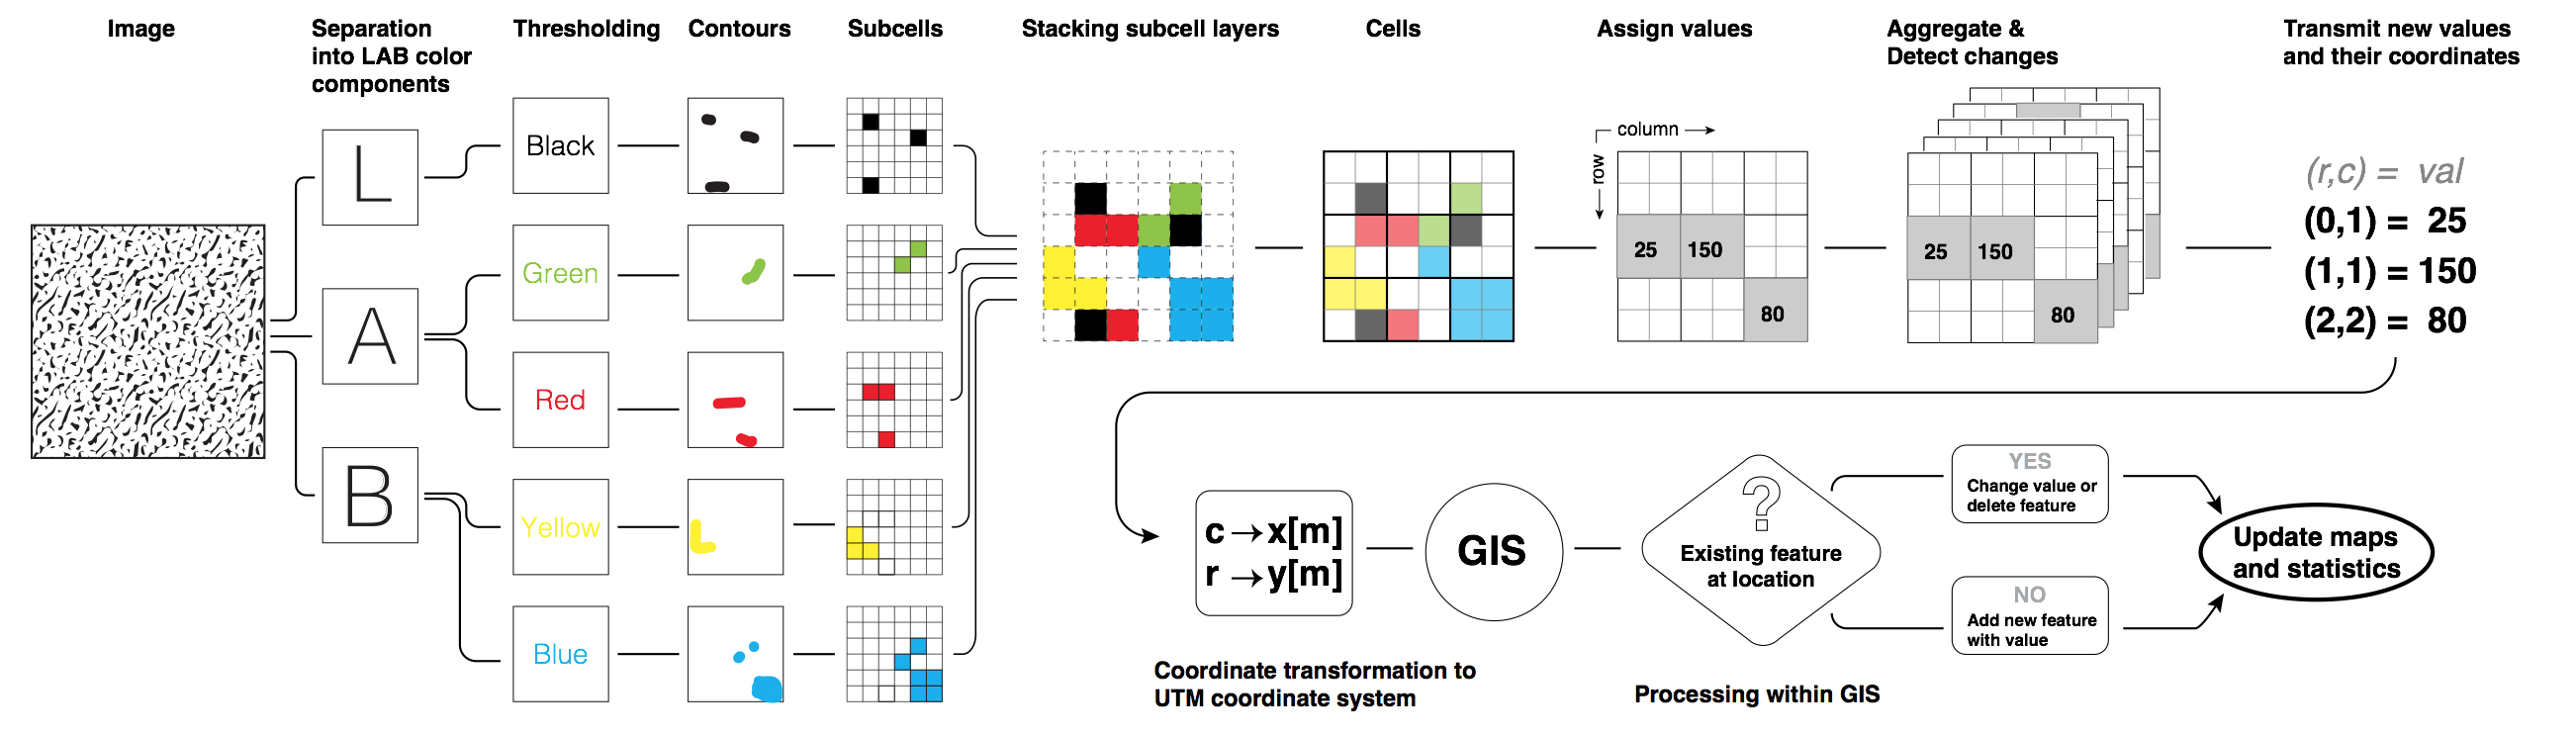
\includegraphics[width=1\textwidth]{chapters/consensus/findingplaces/figures/fp7.png}
                \end{center}
                \caption{FindingPlaces TUI Scanning Module: Processing of a video frame to GIS query. FindingPlaces utilized 4 webcams to capture the overall table state; The captured image would then be processed to allocate colored tiles, and project them onto a geographic coordination system. Finally, tiles found to match a designated site would add or subtract housing capacity in that area, thus affecting the overall housing count.}
                \label{fig:predictions_scan}
            \end{figure}

            the TUI utilized few regularly shaped, color-coded LEGO tiles on a plexiglass grid \eqref{subsec:csarch-cityscopy}. All other grid cells were filled with low, neutrally white objects that provided a canvas for the map display via the overhead projectors. In order to scan the entire surface of the CityScope TUI simultaneously, an array of four web-cameras was used, each one covering a square quarter of the table. Image recognition was handled by two single-board mini-computers which streamed the video from the webcams to a workstation computer. The single-board scanning units ran \texttt{ffserver} and \texttt{ffmpeg} to stream their video feeds to the network. Video processing and interpretation were implemented using the computer vision library \texttt{OpenCV} and \texttt{numpy} \cite{opencv_library}.
            \newline
            Shapes visible in the webcam video feed were then analyzed and compared against a lookup table of known brick color-codes. The data attributes and coordinates of successfully detected bricks were then transmitted and translated it into the GIS context. The GIS server was then queried for the attributes of the bricks, computed the new state, and displayed the results on the different output devices. Figure \eqref{fig:predictions_scan} illustrates the scanning process and GIS geo-projection.
        }

        \subsubsection{Software}
        {
            The specialized software for the FP project included microservice-like architecture. The majority of communication between processes was handled using a publish-subscribe pattern built on a Crossbar router with \texttt{Autobahn.JS} and \texttt{Autobahn-Python} clients using WebSockets for asynchronous processing. The main GIS server was a GeoServer instance, with its data managed in a \texttt{PostgreSQL} and \texttt{PostGIS} database. Map display on the tables was done via OpenLayers clients in web-browser windows. Data transfer and spatial queries between the GIS server and the clients were performed via GeoServer's \texttt{WFS API} using the Python bindings of OGR/GDAL, while specific non-spatial queries were run directly against the database. The backend was developed in Python, and the frontend with standard web technologies \texttt{JavaScript, HTML, and CSS}.
        }

    }

    \subsection{Participation Campaign}
    {
        Between May and July 2016, a total of 34, two-hour workshops were held at HafenCity University campus, totalling nearly 400 participants. Each workshop focused on one of the city's seven districts, and participants were specifically invited based on their prior knowledge of these areas. The workshops were advertised via various media channels and $\sim$40,000 brochures distributed all over the city, having an estimated reach of $\sim$5 million citizens. Participants were asked to register online and $\sim$20 people per session were eventually invited; On average, 11 people participated per workshop. Participants could only attend one workshop per district, while response and registration numbers varied based on each district. The diverse range of participants was characterized by a strong heterogeneity concerning age, profession, political views, social values, and personal motivation to participate.


        \begin{figure}[!htb]
            \begin{center}
                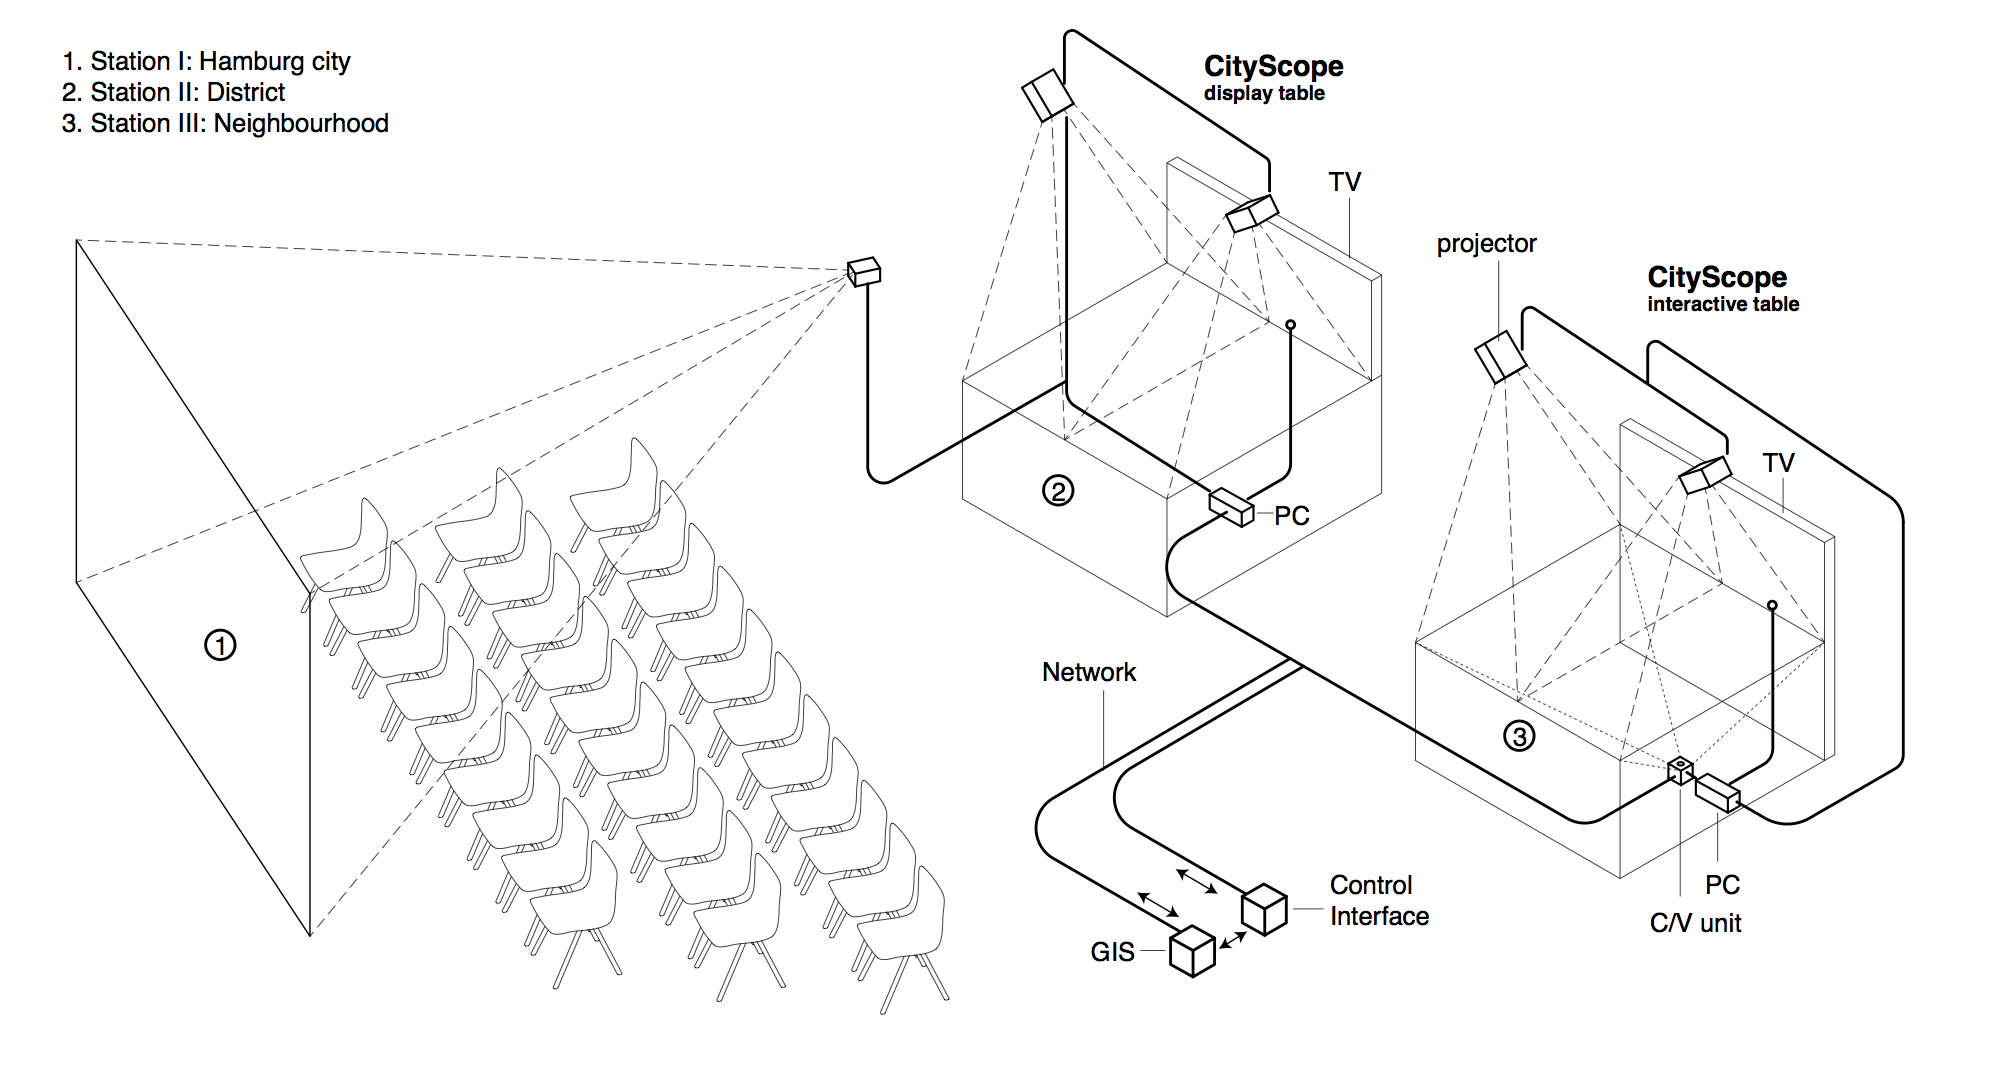
\includegraphics[width=1\textwidth]{chapters/consensus/findingplaces/figures/fp8.png}
            \end{center}
            \caption{FindingPlaces - CityScope Setup. Amongst other contributions, FindingPlaces was the first interconnected CityScope system that linked user-interactions and data from multiple instances, and utilized it in all other places. This created a sense of continuation between the different Stations, as participants could observe their previous actions reflected in other stations.}
            \label{fig:predictions_setup_overall}
        \end{figure}

        \subsubsection{Venue and Moderation}
        {
            The workshops took place from Monday to Saturday at a gallery space of 150$m^2$ on HCU entrance floor. This site was deliberately chosen for being considered a neutral location in the city for the often emotionally charged discussions on refugee accommodations. A team of six to eight people was in charge of the organization and conduct of each workshop: one moderator leading the discussion, one assistant documenting the exchange, one researcher accompanying the workshops for scientific purposes, one technical staff operating the equipment, and one or two representatives each from the Central Refugees Coordination Staff and district administration. The moderators were leading the workshops, while other team members provided on-demand details concerning the CityScope system, specific sites, or information regarding refugees' accommodation in general. In later review, it was mentioned that the open discussion contributed to the participants' grasp of the complex subject matter. Figures \eqref{fig:fp_session} and \eqref{fig:predictions_setup_overall} show a typical workshop setup at the HCU venue.
        }
    }

    \subsection{Workshop Procedure}
    {
        Similar to the BRT project \eqref{sec:brt}, the venue was divided into three stations, displaying different scales of the city: Hamburg City region, district, and neighborhood.

        \subsubsection{(i) Hamburg City}
        {
            At first, an intro video was shown to inform participants about the workshop procedure, the current condition of refugees, and the challenge of providing appropriate accommodation. The general task was presented: `Which city-owned parcels would be suitable locations for refugee accommodation?' The goal was to find sites that in total could accommodate nearly 20,000 refugees and thus meet the predicted demand until the end of 2016\footnote{Total predicted newcomers varied significantly during 2015-2016. Geopolitical shifts, such as border closures and stricter migration control in eastern states changed Hamburg's predictions over time \cite{katz2016cities}. Nevertheless, the goal of FP was to build a pool of sites not only for current newcomers, but also for potential future ones.}. The locations of all existing and planned refugee accommodations were shown on a map, as well as the current statistics on the refugee distribution to the different districts. In addition, the targeted number of accommodation places was displayed, counting down in real-time in response to new locations proposed by the participants during the workshops.
        }

        \begin{figure}[!htb]
            \begin{center}
                \includegraphics[width=1\textwidth]{chapters/consensus/findingplaces/figures/fp2.png}
            \end{center}
            \caption{
                Regional and District Scales. This CityScope instance showed the locations of existing and planned refugee accommodations, including their actual occupation rates were indicated. Available places were colored: $Red$ for places with a high indication of unsuitability, $orange$ for a medium indication, and $yellow$ for likely suitable places. Further information on the number of inhabitants and refugees currently accommodated in the district was presented on a screen.
            }
            \label{fig:fp_city_scale}
        \end{figure}


        \subsubsection{(ii) District}
        {
            After the introduction, the first CityScope table was introduced. Here, a satellite image projected onto the table showed the city district at stake. Street and neighborhood names, as well as distinctive points of interest, were displayed to provide orientation. As with the city scale, the locations of existing and planned refugee accommodations, including their actual occupation rates were indicated. Available places were colored according to their previously determined suitability classes: $Red$ for places with a high indication of unsuitability, $orange$ for a medium indication, and $yellow$ for likely suitable places. Further information on the number of inhabitants and refugees currently accommodated in the district was presented on a screen. Taking into account that not all spaces could possibly be discussed during the two-hour workshop, the participants were asked to select focus-areas for the next station. Selection criteria could be specific knowledge of a place, the need for equal distribution of refugees within the city, or the color-index of the spaces. Figure \eqref{fig:fp_city_scale} shows the locations of existing and planned refugee accommodations, as well as areas which can be considered for allocation of new housing.
        }


        \begin{figure}[!htb]
            \begin{center}
                \includegraphics[width=1\textwidth]{chapters/consensus/findingplaces/figures/fp5.png}
            \end{center}
            \caption{
                Neighborhood Scale. After observing the regional scale, a chosen focus area was projected on an interactive CityScope, in which participants were able to identify details such as buildings, parks or playgrounds. By placing a marker piece onto a parcel, the potential accommodation capacity for the site was indicated. Additionally, area in $m^2$, planning regulations, and restrictions such as nature conservation, biotope, or high-voltage lines, were presented. When participants reached a consensus and identify a location suitable for refugee accommodation, another marker piece was placed on the TUI, indicating the number of accommodation places (40 - 1,500); the screens and the CityScope at the Hamburg and district-stations were also displaying the location of the suggested parcel. Photo: W. Schieswohl, author.
            }
            \label{fig:fp_neighborhood_scale}
        \end{figure}


        \subsubsection{(iii) Neighborhood}
        {
            The chosen focus areas were projected onto the second interactive CityScope, with the suitability classes shown in colored hatching. At this scale, participants were able to identify details like buildings, parks or playgrounds. In addition to refugee accommodations, social infrastructure like kindergartens or schools, as well as bus or train stops was shown. By placing a marker piece onto a parcel, detail information on the property was displayed on a screen, including area in $m^2$, planning regulations, designation of the area, as well as restrictions such as nature conservation, biotope, or high-voltage lines. Additionally, the potential accommodation capacity for the site was computed and indicated. Participants' verbal discussion of the pros and cons for each parcel were logged and displayed on the screen.
            \newline
            When participants reached a consensus and identify a location suitable for refugee accommodation, this parcel could be suggested and forwarded to the city officials. To do so, another marker piece was placed on the TUI, indicating the number of accommodation places (between 40 to 1,500). At that point, the screens and the CityScope at the Hamburg and district-stations were also displaying the location of the suggested parcel. Finally, the proposed number of refugees was included in the system's statistics. Figure \eqref{fig:fp_neighborhood_scale} shows the interaction with the Neighborhood Scale TUI.
        }
    }

    \subsection{Results}
    {

        \begin{figure}[!htb]
            \begin{center}
                \includegraphics[width=1\textwidth]{chapters/consensus/findingplaces/figures/fp1.png}
            \end{center}
            \caption{FindingPlaces results. (top) The map marks the total places found by community members. The colors present `suggested to approval' (blue), `to be further investigated' (yellow), or `not suitable' (red). Importantly, the map demonstrates the rather equal distribution of places found by the general public, which solidifies the sense of general acceptance of asylum seekers amongst diverse neighborhoods. (bottom) Breakdown of results per each administrative district. Photo: FindingPlaces, HCU}
            \label{fig:fp_results}
        \end{figure}

        At the end of each workshop, a list of the agreed upon parcels was delivered directly to the Central Refugees Coordination Staff, along with all information regarding the planning restrictions and transcripts of the discussion. These materials were also uploaded to the official FP website for public access. The Central Refugees Coordination Staff would then initiate a screening process, in which each suggested parcel went through a rigorous feasibility test. The results of this process were published online within two weeks; Parcels which were deemed suitable were then further studied by the city's planning authorities.

        \subsubsection{Allocated Sites}
        {
            In total, 161 locations were suggested by the participants and evaluated by the authorities. With these, accommodation solutions for nearly 24,000 refugees were proposed, exceeding the initial targeted goal of 20,000. More than half of the parcels were designated parks, green areas in inner-city locations, landscape, or agricultural spaces in rural areas, that are mostly subject to nature or landscape conservation. Another 15\% of the suggested parcels were used as sports fields or playgrounds. Others were parking lots, commercial and industrial areas, parcels designated for future housing projects or port area parcels. Almost three quarters of the suggested locations were rated as not suitable in the initial assessment, leaving 44 rated as feasible. A further 24 were excluded after a detailed examination. Ultimately, 6 received recommendations for implementation and 10 were taken into consideration for future planning. In these lasting 6 locations, approximately 750 refugees could be accommodated, 4\% of the initial target. Figure \eqref{fig:fp_results} shows the places found across the regional area of Hamburg, and a breakdown of the results per district.
            \newline
            Several reasons led to rejections of allocated sites: More than a third of the parcels were not available due to the existence of other land-uses, such as commercial activities or sport and leisure purposes. Another third of the parcels could not be used due to direct conflicts of land-use, mostly parks and playgrounds. Other reasons for rejection were of technical or structural nature, such as hazardous environment, contamination, topographic constraints, protection of historical monuments, or a lack of nearby transit and social infrastructure.
        }

        \subsubsection{Interaction Process}
        {
            The FP workshop methodology motivated a high degree of involvement and direct discussion between experts and non-experts. Despite the emotional charge and heated public debate concerning refugee accommodations, the discussions and atmosphere in the workshops were mostly constructive. Occasionally, participants expressed their dissatisfaction with the refugee policy pursued by the Hamburg senate. Some were arguing that FP might have been a dishonest participation process, only utilized to restore peace in the city.
            \newline
            However, it could be observed that the disapproving comments were mostly based on vague or incorrect information, and were hence quickly diminishing with the provision of more precise information. This highlighted that the dialogue between the participants could be quickly rationalized by shifting from a theoretical discussion to a more tangible level, through the usage of clear information and facts. For example, participants could not simply reject a proposed parcel without providing arguments that were clear to other participants. During the workshops, many ideas of an ideal solution for refugees accommodation had to pass a `reality check', pushing some to be revised as they were incompatible with the applicable planning regulations and site restrictions.
        }
    }

    \begin{figure}[!htb]
        \begin{center}
            \includegraphics[width=1\textwidth]{chapters/consensus/findingplaces/figures/fp3.png}
        \end{center}
        \caption{
            Participation and engagement. As with the Boston BRT project \eqref{sec:brt}, the FindingPlaces CityScope's were designed as a literal common-ground, in which technology is only set to encourage a vibrant public discourse. The tables were sized to accommodate a large number of participants, and the groups were able to interact freely with the system. Extra effort was made to ensure disabled and elderly participants were not disadvantaged; Nevertheless, the system presented a degree of visual complexity not always suitable for the general public. Photo: W. Schieswohl, City of Hamburg, HCU.
        }
        \label{fig:fp_engagement}
    \end{figure}

    \subsection{Discussion}
    {
        By both stakeholders and participants, FP was evaluated as a highly positive experience, and CityScope was recognized to greatly support public participation and real-time decision-making. It was noted that citizens felt as partners in an `eye-level' dialogue with policy-makers and city administration, being able to supply planning authorities with relevant information based on their local knowledge. The project built up acceptance towards refugee accommodation in Hamburg, and triggered high-quality feedback in comparison to other public discussions at the time. Making administrative procedures and decisions transparent effectively contributed to the `political literacy' of the general citizenship.

        \subsection{Limitations}
        {
            A key challenge of FP was the tight schedule in which the project needed to be implemented and communicated to the general public. Logistical limitations reduced the overall exposure of the CityScope tool: Due to the size of the platform, workshops were bound to be held at HCU campus instead of closer to participants' locations. This naturally reduced the number of potential participants, thus contributing to a selection bias which favored more mobile and capable members of the community \cite{Innes2016}.
            \newline
            Another constrain was the form of representation of urban data: Despite thorough pre-processing, non-expert participants had trouble understanding the professional planning content, which was not distilled enough for the general public. As participants were not used to working with maps or satellite images, orienting the projected images and assessing them adequately was challenging. Figure \eqref{fig:fp_engagement} shows the engagement of participants in the workshop, and the potential complexity of the FP data visualization.
            \newline
            Lastly, sites that were eventually deemed unsuitable, were not immediately removed from the system, but rather were evaluated by the planning authorities at a later stage. This meant that the system was not able to provide a clear picture of the feasibility of proposed sites in real-time, thus reducing the number of sites that were eventually approved. In future versions of such system, pre-approval or rejection of simple sites (i.e., sites with clear feasibility indication) should be automated.
        }
    }

    \subsection{Conclusion}
    {
        Refugees and global immigration waves remain a major challenge of high urgency all across the world. Global socio-political developments may yield new migrant waves, and the accommodation of refugees in `arrival cities' remains acute. The usage of CityScope in this context, demonstrated how socio-technical platforms can effectively support consensus-building and trust amongst the public. It highlighted the importance of gaining `street-knowledge' and crowd-sourced perspective, while validating it with facts, data, and information. CityScope served this project in two ways: It assisted with fast and accurate decision-making, by methodically allocating and evaluating housing solutions. But more broadly, CityScope FP was acting as an amplifier which echoed the public's voice, helping them to collectively discuss, design, and shape their own urban future.
    }
}